\documentclass[conference]{IEEEtran}
\IEEEoverridecommandlockouts

\usepackage{cite}
\usepackage{amsmath,amssymb,amsfonts}
\usepackage{algorithmic}
\usepackage{algorithm}
\usepackage{graphicx}
\usepackage{textcomp}
\usepackage{xcolor}
\usepackage{tikz}
\usepackage{booktabs}
\usepackage{array}
\usepackage{url}

\usetikzlibrary{arrows.meta,positioning,shapes.geometric,calc,fit,backgrounds}

\begin{document}

\title{BreachShield: AI Powered OSINT Breach Detection \& Dark Web Protection}

\author{
\IEEEauthorblockN{Arvind D. H., Girishkumar N. M., Manoj, Premkumar Teli}
\IEEEauthorblockA{\textit{Department of Information Science and Engineering} \\
\textit{Acharya Institute of Technology}, Bengaluru, India}
\and
\IEEEauthorblockN{Sushma T. M.}
\IEEEauthorblockA{\textit{Assistant Professor, Dept. of Information Science and Engineering} \\
\textit{Acharya Institute of Technology}, Bengaluru, India}
}

\maketitle

\begin{abstract}
Breach notification and dark-web exposure intelligence platforms suffer from a fundamental privacy paradox: to determine whether personal credentials have been compromised, users must transmit those sensitive identifiers in plaintext to a third-party server, creating a centralized query-surveillance and correlation vector. This paper presents BreachShield, a privacy-preserving Open-Source Intelligence (OSINT) breach detection and threat assessment platform designed to resolve this tension through cryptographic query isolation, accountable gating, and verifiable audit logging. BreachShield combines a client-side $k$-anonymity range-query protocol (20-bit SHA-256 prefix partitioning) executed via the W3C Web Crypto API, a dual-channel out-of-band One-Time Password (OTP) identity gate, a pluggable OSINT source aggregation engine supporting live breach stores and Telegram scraping, an empirical machine-learning breach severity assessment framework, and a Merkle-tree batched audit trail anchored to an Ethereum Virtual Machine (EVM) smart contract. We define a comprehensive threat model spanning external eavesdroppers, malicious authenticated users, insider adversaries, and source-poisoning vectors, supported by formal security and privacy analyses that evaluate prefix leakage against Private Set Intersection (PSI) baselines. We report extensive functional evaluation across all pipeline subsystems and detail the experimental evaluation of a 165-dimensional gradient-boosted decision tree classifier (XGBoost, 89.2\% test accuracy) benchmarked against deep learning architectures.
\end{abstract}

\begin{IEEEkeywords}
Breach intelligence, $k$-anonymity, Open-Source Intelligence (OSINT), threat modeling, Merkle tree, blockchain audit log, XGBoost, query privacy.
\end{IEEEkeywords}

\section{Introduction}
The exponential expansion of digital identity surfaces and automated credential theft has precipitated widespread exfiltration of personal records onto dark-web marketplaces, underground paste sites, and public data dumps \cite{aljofey2020effective,kuhn2024navigating}. Traditional compromise-checking services are fundamentally reactive and architecturally centralized. Users or corporate security teams seeking to determine credential exposure typically submit target queries---such as cleartext email addresses, employee identities, or telephone numbers---directly to centralized lookup services. This lookup process exposes users to third-party query tracking: the lookup provider learns precisely which identifier is being monitored, when the query occurred, and the requesting network location \cite{li2019protocols}. Consequently, querying for compromised status inadvertently creates a high-value surveillance vector.

To counteract query-exposure risks, partial prefix-matching constructions (commonly termed $k$-anonymity range queries) have been introduced \cite{sweeney2002k,li2019protocols}. In these models, clients hash target identifiers locally and submit only a truncated cryptographic hash prefix. The lookup server returns all records matching that prefix bucket, leaving the final matching step to the client. While prefix disclosure prevents the server from deterministically identifying the requested record among bucket candidates, naive public range endpoints remain vulnerable to bulk enumeration and dictionary-scraping attacks. Malicious actors can traverse the finite prefix space ($16^d$ possibilities) to harvest complete compromised credential corpora.

Furthermore, multi-source OSINT threat ingestion introduces acute data integrity and operational reliability challenges \cite{kuhn2024navigating}. Underground data sources, such as distributed Telegram dump channels, operate with erratic uptime, rate limits, and unauthenticated provenance. Once compromise intelligence is obtained, security administrators face the operational challenge of triaging threat severity: distinguishing between low-impact leaks (e.g., outdated usernames) and critical exposures (e.g., plaintext passwords correlated with national identity records). Finally, audit records generated during organizational investigations are vulnerable to retroactive manipulation or repudiation by privileged insiders unless backed by cryptographic integrity guarantees \cite{crosby2009efficient,arabnouri2024secure}.

This paper presents BreachShield, a privacy-preserving OSINT breach intelligence platform engineered to address query privacy, authenticated enumeration resistance, multi-source aggregation, severity triage, and audit integrity within a unified architecture. BreachShield implements an end-to-end operational pipeline combining client-side Web Crypto SHA-256 partitioning, an out-of-band carrier-compliant OTP authentication gate, concurrent OSINT source dispatching, heuristic and machine-learning threat scoring, and Merkle-tree batched EVM smart contract anchoring.

The contributions of this paper are:
\begin{enumerate}
    \item \textbf{Privacy-Preserving Breach Intelligence Architecture:} A client-side $k$-anonymity range-query protocol that bounds query disclosure to 20 bits of entropy, performing local cryptographic partitioning via the W3C Web Crypto API prior to network transmission.
    \item \textbf{Multi-Source OSINT Aggregation Framework:} An extensible asynchronous provider pipeline featuring concurrent dispatching, thread-safe Telegram scraper microservices with mutex-controlled SQLite session pooling, and automated failover data stores.
    \item \textbf{OTP-Gated Authenticated Breach-Search Architecture:} An accountable access control gate utilizing cryptographically secure OTP issuance, bcrypt hashing, carrier-compliant telecom DLT SMS templating via an Android gateway, and cryptographic session-token binding that enforces identity match invariants.
    \item \textbf{Tamper-Evident Audit Logging:} A deterministic audit logger using sorted-key canonical JSON leaf hashing, asynchronous batch buffering (100-record / 60-second window), Merkle tree generation, and EVM smart contract state anchoring.
    \item \textbf{Experimental Machine-Learning Severity Assessment:} An empirical benchmark evaluating XGBoost against 1D-CNN, RNN, and Transformer architectures across 1,034 curated breach records on a 165-dimensional feature space, establishing structural criteria for tabular exposure triage.
\end{enumerate}

% ====================================================================
% SECTION II: THREAT MODEL
% ====================================================================
\section{Threat Model}

\begin{figure*}[!t]
\centering
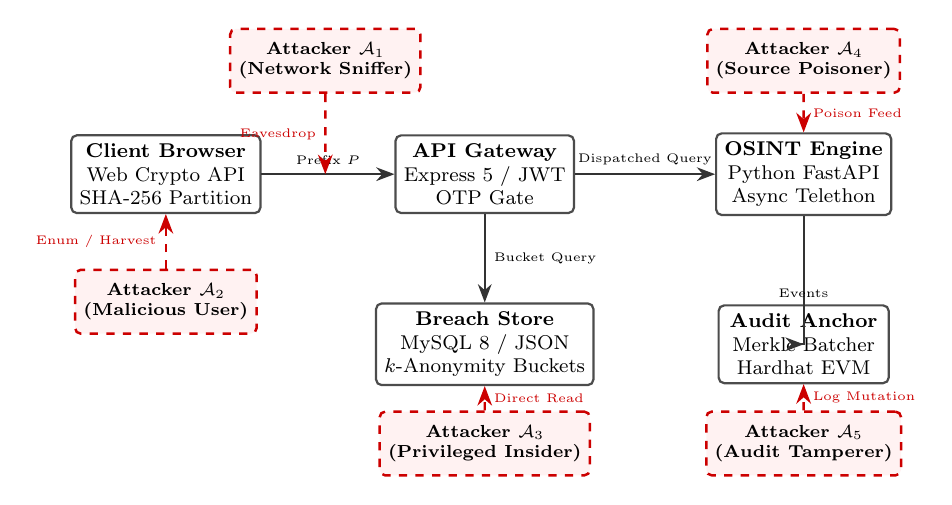
\begin{tikzpicture}[
    scale=0.9, every node/.style={transform shape},
    box/.style={draw=black!70, rounded corners=2pt, minimum width=2.4cm, minimum height=1.0cm, align=center, font=\footnotesize, fill=white, line width=0.8pt},
    threatbox/.style={draw=red!80!black, dashed, rounded corners=2pt, minimum width=2.2cm, minimum height=0.9cm, align=center, font=\scriptsize\bfseries, fill=red!5, line width=0.9pt},
    zone/.style={draw=blue!40!black, dotted, rounded corners=4pt, inner sep=6pt, fill=blue!2, line width=0.7pt},
    arrow/.style={-{Stealth[scale=1.0]}, line width=0.8pt, draw=black!80},
    tarrow/.style={-{Stealth[scale=1.0]}, line width=0.9pt, draw=red!80!black, dashed}
]
    % Threat Zones
    \node[box] (client) at (0, 3.2) {\textbf{Client Browser}\\Web Crypto API\\SHA-256 Partition};
    \node[box] (gateway) at (4.5, 3.2) {\textbf{API Gateway}\\Express 5 / JWT\\OTP Gate};
    \node[box] (fastapi) at (9.0, 3.2) {\textbf{OSINT Engine}\\Python FastAPI\\Async Telethon};
    \node[box] (storage) at (4.5, 0.8) {\textbf{Breach Store}\\MySQL 8 / JSON\\$k$-Anonymity Buckets};
    \node[box] (ledger) at (9.0, 0.8) {\textbf{Audit Anchor}\\Merkle Batcher\\Hardhat EVM};

    % Attackers
    \node[threatbox] (adv_ext) at (2.25, 4.8) {Attacker $\mathcal{A}_1$\\(Network Sniffer)};
    \node[threatbox] (adv_enum) at (0, 1.4) {Attacker $\mathcal{A}_2$\\(Malicious User)};
    \node[threatbox] (adv_ins) at (4.5, -0.6) {Attacker $\mathcal{A}_3$\\(Privileged Insider)};
    \node[threatbox] (adv_src) at (9.0, 4.8) {Attacker $\mathcal{A}_4$\\(Source Poisoner)};
    \node[threatbox] (adv_log) at (9.0, -0.6) {Attacker $\mathcal{A}_5$\\(Audit Tamperer)};

    % Legitimate Paths
    \draw[arrow] (client) -- node[above, font=\tiny] {Prefix $P$} (gateway);
    \draw[arrow] (gateway) -- node[above, font=\tiny] {Dispatched Query} (fastapi);
    \draw[arrow] (gateway) -- node[right, font=\tiny] {Bucket Query} (storage);
    \draw[arrow] (fastapi) |- node[near start, below, font=\tiny] {Events} (ledger);

    % Threat Vectors
    \draw[tarrow] (adv_ext) -- node[left, font=\tiny, text=red!80!black] {Eavesdrop} (2.25, 3.2);
    \draw[tarrow] (adv_enum) -- node[left, font=\tiny, text=red!80!black] {Enum / Harvest} (client);
    \draw[tarrow] (adv_ins) -- node[right, font=\tiny, text=red!80!black] {Direct Read} (storage);
    \draw[tarrow] (adv_src) -- node[right, font=\tiny, text=red!80!black] {Poison Feed} (fastapi);
    \draw[tarrow] (adv_log) -- node[right, font=\tiny, text=red!80!black] {Log Mutation} (ledger);

\end{tikzpicture}
\caption{Threat model and adversarial attack surface across the BreachShield operational pipeline.}
\label{fig:threat_model}
\end{figure*}

\subsection{System Assets and Security Assumptions}
The assets requiring protection within BreachShield include:
\begin{itemize}
    \item \textbf{Target Identifier Privacy ($T$):} The plaintext identity (email address or phone number) queried by a user.
    \item \textbf{Credential Integrity:} The authoritative repository of breach metadata and suffix buckets.
    \item \textbf{Audit Log Verifiability:} The chronological record of compliance events and threat intelligence queries.
    \item \textbf{Authentication Credentials:} Ephemeral OTP codes, bcrypt password hashes, and JSON Web Tokens (JWT).
\end{itemize}
We assume all operational communication between browser clients, the API gateway, microservices, and external carriers occurs over TLS 1.3. Cryptographic primitives including SHA-256 and bcrypt are assumed computationally secure against preimage and collision attacks.

\subsection{Adversary Taxonomy and Capabilities}
We define five adversarial classes categorized by vantage point and capabilities, as illustrated in Fig.~\ref{fig:threat_model}.

\subsubsection{Attacker $\mathcal{A}_1$ (External Network Adversary)}
An active adversary positioned on the network path between the client browser and the API gateway. $\mathcal{A}_1$ can eavesdrop on, intercept, replay, or inject arbitrary packets. We assume TLS 1.3 prevents payload interception and modification; however, $\mathcal{A}_1$ observes packet timing, transfer volumes, and TLS SNI metadata.

\subsubsection{Attacker $\mathcal{A}_2$ (Authenticated Malicious User)}
A legitimate user who successfully completes OTP verification for an identifier $T_A$ but seeks to: (i) harvest prefix buckets to reconstruct the server-side breach corpus; (ii) execute queries against unauthorized third-party identifiers $T_B \ne T_A$; or (iii) exhaust downstream OSINT feed rate limits via request flooding.

\subsubsection{Attacker $\mathcal{A}_3$ (Malicious or Compromised Insider)}
An adversary possessing administrative read access to backend application servers, runtime process memory, and the persistent MySQL storage layer. $\mathcal{A}_3$ attempts to correlate client IP addresses, JWT tokens, and requested prefix buckets to reconstruct plaintext user search targets.

\subsubsection{Attacker $\mathcal{A}_4$ (Source-Poisoning Adversary)}
A malicious external entity controlling an upstream intelligence channel (such as a monitored public Telegram dump or simulated breach paste). $\mathcal{A}_4$ injects malformed data, deceptive entity records, or denial-of-service payloads into ingestion streams to corrupt threat triage scoring.

\subsubsection{Attacker $\mathcal{A}_5$ (Audit Log Adversary)}
A privileged adversary attempting to retroactively delete, truncate, reorder, or manipulate query audit logs to conceal unauthorized lookups or falsify historical evidence.

% ====================================================================
% SECTION III: SYSTEM ARCHITECTURE
% ====================================================================
\section{System Architecture \& Implementation}

BreachShield is structured as a decoupled, multi-tier microservice architecture consisting of a React 19 web client, an Express 5 API gateway, a Python FastAPI OSINT microservice, an Android Kotlin SMS relay gateway, and an EVM smart contract anchor registry (Fig.~\ref{fig:sys_arch}).

\begin{figure*}[!t]
\centering
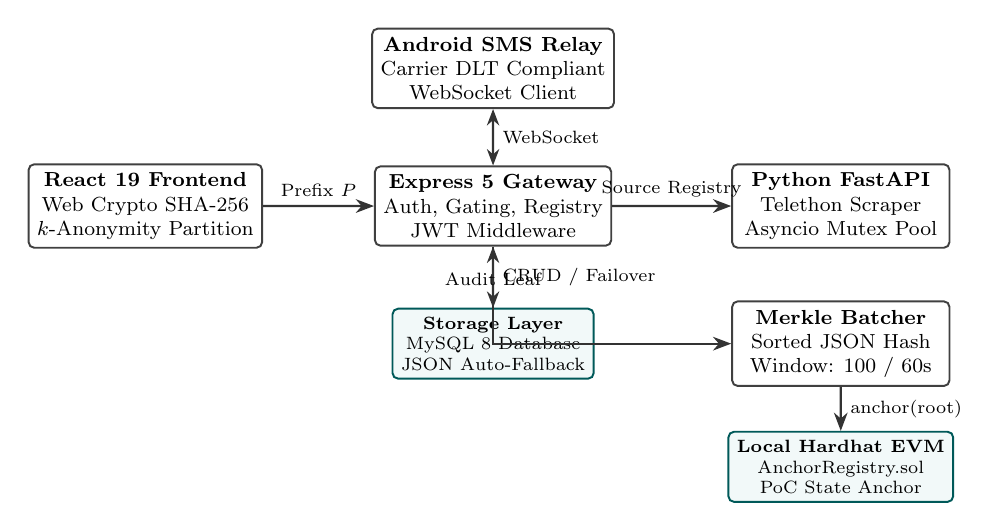
\begin{tikzpicture}[
    scale=0.92, every node/.style={transform shape},
    tier/.style={draw=blue!60!black, fill=blue!4, rounded corners=3pt, line width=0.8pt, inner sep=6pt},
    comp/.style={draw=black!75, fill=white, rounded corners=2pt, minimum width=3.0cm, minimum height=0.85cm, align=center, font=\footnotesize, line width=0.7pt},
    data/.style={draw=teal!70!black, fill=teal!5, rounded corners=2pt, minimum width=2.6cm, minimum height=0.75cm, align=center, font=\scriptsize, line width=0.7pt},
    arrow/.style={-{Stealth[scale=1.0]}, line width=0.8pt, draw=black!80},
    darrow/.style={{Stealth[scale=0.9]}-{Stealth[scale=0.9]}, line width=0.8pt, draw=black!80}
]
    % Client Tier
    \node[comp] (react) at (0, 2.5) {\textbf{React 19 Frontend}\\Web Crypto SHA-256\\$k$-Anonymity Partition};
    
    % Gateway Tier
    \node[comp] (gateway) at (4.8, 2.5) {\textbf{Express 5 Gateway}\\Auth, Gating, Registry\\JWT Middleware};
    \node[comp] (android) at (4.8, 4.4) {\textbf{Android SMS Relay}\\Carrier DLT Compliant\\WebSocket Client};
    \node[data] (mysql) at (4.8, 0.6) {\textbf{Storage Layer}\\MySQL 8 Database\\JSON Auto-Fallback};

    % OSINT Engine
    \node[comp] (fastapi) at (9.6, 2.5) {\textbf{Python FastAPI}\\Telethon Scraper\\Asyncio Mutex Pool};
    
    % Anchoring Tier
    \node[comp] (batcher) at (9.6, 0.6) {\textbf{Merkle Batcher}\\Sorted JSON Hash\\Window: 100 / 60s};
    \node[data] (contract) at (9.6, -1.1) {\textbf{Local Hardhat EVM}\\AnchorRegistry.sol\\PoC State Anchor};

    % Connections
    \draw[arrow] (react) -- node[above, font=\scriptsize] {Prefix $P$} (gateway);
    \draw[darrow] (gateway) -- node[right, font=\scriptsize] {WebSocket} (android);
    \draw[darrow] (gateway) -- node[right, font=\scriptsize] {CRUD / Failover} (mysql);
    \draw[arrow] (gateway) -- node[above, font=\scriptsize] {Source Registry} (fastapi);
    \draw[arrow] (gateway) |- node[near start, above, font=\scriptsize] {Audit Leaf} (batcher);
    \draw[arrow] (batcher) -- node[right, font=\scriptsize] {anchor(root)} (contract);

\end{tikzpicture}
\caption{BreachShield multi-tier system architecture and operational data paths.}
\label{fig:sys_arch}
\end{figure*}

\subsection{Client-Side Anonymization Tier}
The presentation tier is implemented in React 19. Plaintext targets $T$ are normalized locally by lowercasing and trimming whitespace. The normalized string is transformed into a 256-bit hash $H = \text{SHA-256}(T)$ using the browser's hardware-accelerated W3C Web Crypto API (\texttt{frontend/src/lib/kAnonymity.js}). $H$ is represented as a 64-character hexadecimal string, split into a 5-character (20-bit) prefix $P = H[0:5]$ and a 59-character (236-bit) suffix $S = H[5:64]$. The plaintext target $T$ and the suffix $S$ never traverse the network during range querying.

\subsection{API Gateway \& Session Gating}
The gateway tier runs on Express 5 (\texttt{backend/server.js}). It enforces rate limiting, CORS restrictions, session validation, and breach source registry orchestration. Access to range queries is guarded by the \texttt{verifyOtpToken} middleware, ensuring requests originate from verified sessions. MySQL 8 serves as the persistent store for user records, OTP states, and local breach dumps, with an automatic JSON file-based fallback layer (\texttt{backend/auth/db.js}) activated upon database disconnection.

\subsection{OSINT Ingestion Microservice}
High-entropy dark-web dump tracking is handled by a dedicated Python FastAPI microservice. Integration with Telegram channels uses the Telethon MTProto client library. Because SQLite session files incur file-lock collisions under concurrent asynchronous requests (\texttt{sqlite3.OperationalError}), the microservice serializes channel client access through an \texttt{asyncio.Lock} mutex with an 8.0-second timeout boundary, guaranteeing process isolation.

\subsection{Android Telecom Relay Gateway}
In jurisdictions with strict Distributed Ledger Technology (DLT) telecom mandates (such as India's TRAI regulations), automated cloud SMS gateways drop non-templated OTP payloads. BreachShield integrates a companion Android native client written in Kotlin (\texttt{android-gateway/}). The application establishes a persistent bidirectional WebSocket connection to the Express gateway, receiving pending OTP dispatch requests and transmitting them via carrier hardware using pre-approved SMS header templates.

\subsection{Pluggable Source Registry}
Breach sources implement an abstract contract defined in \texttt{backend/sources/BreachSource.js}:
\begin{equation}
    \text{search}(\text{target}, \text{targetHash}) \to \mathcal{P}(\text{Record})
\end{equation}
The registry dynamically loads four concrete adapters:
\begin{enumerate}
    \item \texttt{PublicBreachSource}: Executes range queries against the local normalized breach database ($k$-anonymity store).
    \item \texttt{TelegramScraperSource}: Dispatches HTTP queries to the FastAPI scraper microservice.
    \item \texttt{PhishingFeedSource}: Pluggable adapter scaffolding for domain reputation feeds.
    \item \texttt{ThreatIntelSource}: Pluggable adapter scaffolding for third-party commercial threat intelligence.
\end{enumerate}
In the operational prototype, \texttt{PublicBreachSource} and \texttt{TelegramScraperSource} execute live queries over real datasets, whereas \texttt{PhishingFeedSource} and \texttt{ThreatIntelSource} remain non-networked stubs for future feed integration.

\subsection{Operational Risk-Scoring Engine}
Threat triage on the operational search path is computed dynamically by \texttt{riskEngine.js: analyzeExposure()} rather than using pre-canned values. The engine executes regular-expression parsing across multi-source textual dumps to extract exposed entity types, accumulating category points:
\begin{itemize}
    \item Document / National ID exposure: up to 35 points.
    \item Password / cryptographic hash material: up to 30 points.
    \item Physical address coordinates: up to 20 points.
    \item Phone numbers: up to 15 points.
    \item Multiple independent source mentions: up to 15 points.
\end{itemize}
Additionally, the engine computes cross-record correlation scores by evaluating shared identifier pairs across distinct source records (up to 15 points) and factors in live URL phishing classification probabilities (up to 30 points) inspired by contemporary neural detection baselines \cite{sahingoz2024dephides,pavani2024enhancing,tawfik2025explainable}. The aggregated raw score is floored at 20 (guaranteeing non-zero severity for any confirmed leak), capped at 100, and mapped to categorical severity tiers: \texttt{LOW} ($<40$), \texttt{MEDIUM} ($40$--$59$), \texttt{HIGH} ($60$--$79$), and \texttt{CRITICAL} ($\ge 80$). Recency decay is calculated as:
\begin{equation}
    \omega_{\text{recency}} = \max\left(0.20, \; 1.0 - 0.10 \times (\Delta y)\right)
\end{equation}
where $\Delta y$ is the elapsed time in years since breach occurrence.

% ====================================================================
% SECTION IV: PROTOCOLS
% ====================================================================
\section{Privacy-Preserving Protocols}

\begin{figure*}[!t]
\centering
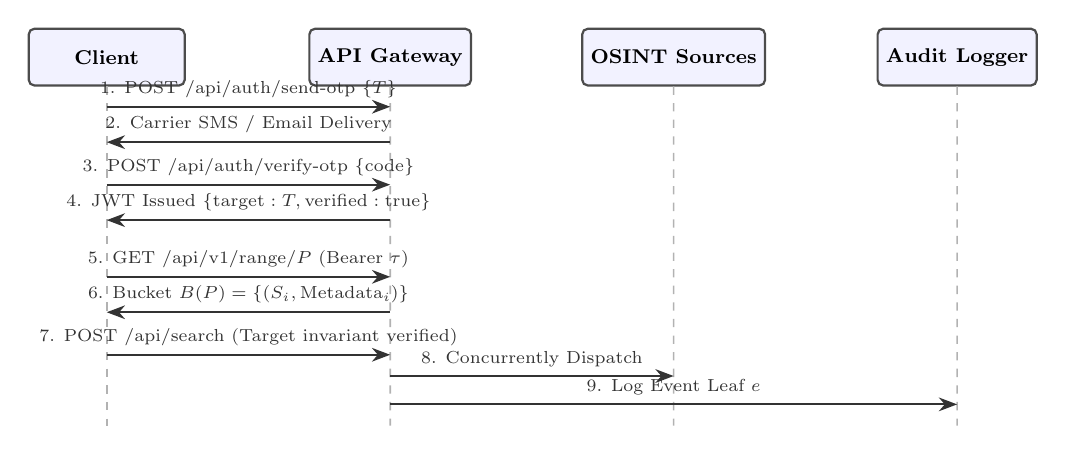
\begin{tikzpicture}[
    scale=0.9, every node/.style={transform shape},
    entity/.style={draw=black!70, fill=blue!5, rounded corners=2pt, minimum width=2.2cm, minimum height=0.8cm, align=center, font=\footnotesize\bfseries, line width=0.8pt},
    arrow/.style={-{Stealth[scale=1.0]}, line width=0.8pt, draw=black!80},
    darrow/.style={{Stealth[scale=0.9]}-{Stealth[scale=0.9]}, line width=0.8pt, draw=black!80},
    note/.style={font=\scriptsize, text=black!80}
]
    % Lifelines
    \node[entity] (client) at (0, 0) {Client};
    \node[entity] (gateway) at (4.0, 0) {API Gateway};
    \node[entity] (sources) at (8.0, 0) {OSINT Sources};
    \node[entity] (audit) at (12.0, 0) {Audit Logger};

    \draw[black!30, dashed, line width=0.6pt] (client) -- (0, -5.2);
    \draw[black!30, dashed, line width=0.6pt] (gateway) -- (4.0, -5.2);
    \draw[black!30, dashed, line width=0.6pt] (sources) -- (8.0, -5.2);
    \draw[black!30, dashed, line width=0.6pt] (audit) -- (12.0, -5.2);

    % Step 1: Send OTP
    \draw[arrow] (0, -0.7) -- node[above, note] {1. POST /api/auth/send-otp $\{T\}$} (4.0, -0.7);
    \draw[arrow] (4.0, -1.2) -- node[above, note] {2. Carrier SMS / Email Delivery} (0, -1.2);

    % Step 2: Verify OTP
    \draw[arrow] (0, -1.8) -- node[above, note] {3. POST /api/auth/verify-otp $\{\text{code}\}$} (4.0, -1.8);
    \draw[arrow] (4.0, -2.3) -- node[above, note] {4. JWT Issued $\{\text{target}: T, \text{verified}: \text{true}\}$} (0, -2.3);

    % Step 3: k-Anonymity Range Query
    \draw[arrow] (0, -3.1) -- node[above, note] {5. GET /api/v1/range/$P$ (Bearer $\tau$)} (4.0, -3.1);
    \draw[arrow] (4.0, -3.6) -- node[above, note] {6. Bucket $B(P) = \{(S_i, \text{Metadata}_i)\}$} (0, -3.6);

    % Step 4: Search & Audit
    \draw[arrow] (0, -4.2) -- node[above, note] {7. POST /api/search (Target invariant verified)} (4.0, -4.2);
    \draw[arrow] (4.0, -4.5) -- node[above, note] {8. Concurrently Dispatch} (8.0, -4.5);
    \draw[arrow] (4.0, -4.9) -- node[above, note] {9. Log Event Leaf $e$} (12.0, -4.9);

\end{tikzpicture}
\caption{Sequence diagram illustrating OTP verification, range query, multi-source search, and audit dispatching.}
\label{fig:search_seq}
\end{figure*}

\subsection{Client-Side $k$-Anonymity Range Query}
BreachShield implements an adapted $k$-anonymity bucket-matching protocol derived from Sweeney's model \cite{sweeney2002k} and popularized by Li et al. \cite{li2019protocols}. Algorithm~\ref{alg:kanonymity} formalizes this procedure.

\begin{algorithm}[!t]
\caption{Client-Side $k$-Anonymity Range Query}
\label{alg:kanonymity}
\begin{algorithmic}[1]
\REQUIRE Target identifier string $T$, verified session token $\tau$
\ENSURE Set of matched breach records $R$
\STATE $T' \leftarrow \text{ToLower}(\text{Trim}(T))$
\STATE $H \leftarrow \text{WebCrypto.SHA-256}(T')$ \COMMENT{Computed in-browser}
\STATE $P \leftarrow H[0:5]$ \COMMENT{20-bit prefix (5 hex chars)}
\STATE $S \leftarrow H[5:64]$ \COMMENT{236-bit suffix (59 hex chars)}
\STATE $B(P) \leftarrow \text{HTTP\_GET}(\text{``/api/v1/range/''} \parallel P, \text{Headers}=\{\text{Bearer } \tau\})$
\STATE $R \leftarrow \emptyset$
\FORALL{$(S_i, \text{Metadata}_i) \in B(P)$}
    \IF{$S_i == S$}
        \STATE $R \leftarrow R \cup \{\text{Metadata}_i\}$
    \ENDIF
\ENDFOR
\STATE \textbf{return} $R$
\end{algorithmic}
\end{algorithm}

The prefix length $d=5$ hex characters defines $16^5 = 1,048,576$ uniform buckets. For a breach catalog containing $N$ records, the expected candidate bucket size is:
\begin{equation}
    E[k] = \frac{N}{16^5} = \frac{N}{1,048,576}
\end{equation}
The mutual information disclosed to the server regarding the full hash $H$ is bounded by:
\begin{equation}
    I(H; P) \le \log_2(16^5) = 20 \text{ bits}
\end{equation}
leaving 236 bits of suffix entropy undisclosed.

\subsection{OTP-Gated Accountable Search Protocol}
To neutralize automated prefix-bucket enumeration by unauthenticated scrapers, BreachShield restricts search endpoints behind a dual-channel OTP gate (\texttt{backend/auth/routes/auth.js}), depicted in Fig.~\ref{fig:search_seq}:
\begin{enumerate}
    \item \textbf{Issuance (\texttt{POST /api/auth/send-otp}):} The gateway enforces a 30-second resend cooldown per target identifier. A six-digit numeric code $C \in [100000, 999999]$ is generated via \texttt{crypto.randomInt()}. The gateway computes a salted bcrypt hash $h_C = \text{bcrypt}(C, 10)$ and stores $(T, h_C, t_{\text{exp}})$ in MySQL with a 5-minute time-to-live ($t_{\text{exp}} = t_{\text{now}} + 300\,\text{s}$). The code is dispatched out-of-band via Nodemailer (email) or the Android DLT SMS gateway (phone).
    \item \textbf{Verification (\texttt{POST /api/auth/verify-otp}):} The client submits candidate code $\hat{C}$. The gateway verifies that fewer than 5 verification attempts have occurred and that $t_{\text{now}} \le t_{\text{exp}}$. Hash equality is validated via \texttt{bcrypt.compare($\hat{C}, h_C$)}.
    \item \textbf{Session Binding:} Upon successful verification, the gateway issues a signed JWT:
    \begin{equation}
        \tau = \text{Sign}_{\text{HMAC-SHA256}}(\{T, \text{verified}: \text{true}\}, K_{\text{jwt}})
    \end{equation}
    with a 1-hour expiration. Range queries and search operations mandate the presence of $\tau$. The gateway strictly enforces an identity invariant:
    \begin{equation}
        \text{normalize}(T_{\text{query}}) \equiv \text{normalize}(\tau.\text{target})
    \end{equation}
    preventing authenticated users from executing lookups against third-party identifiers.
\end{enumerate}

% ====================================================================
% SECTION V: AUDIT LOGGING
% ====================================================================
\section{Tamper-Evident Audit Logging \& Blockchain Anchoring}

\begin{figure}[!t]
\centering
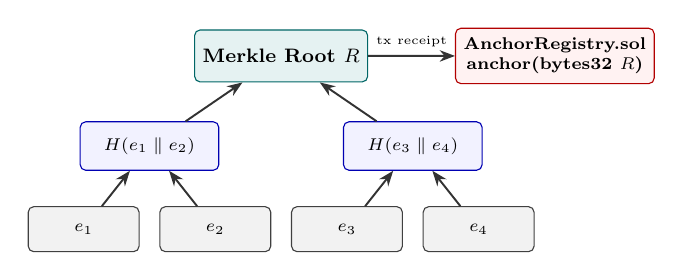
\begin{tikzpicture}[
    scale=0.88, every node/.style={transform shape},
    node distance=0.8cm,
    leaf/.style={draw=black!75, fill=gray!10, rounded corners=2pt, minimum width=1.6cm, minimum height=0.65cm, align=center, font=\scriptsize},
    hashnode/.style={draw=blue!70!black, fill=blue!5, rounded corners=2pt, minimum width=2.0cm, minimum height=0.7cm, align=center, font=\scriptsize\bfseries},
    rootnode/.style={draw=teal!80!black, fill=teal!10, rounded corners=2pt, minimum width=2.4cm, minimum height=0.75cm, align=center, font=\footnotesize\bfseries},
    contract/.style={draw=red!70!black, fill=red!5, rounded corners=2pt, minimum width=2.5cm, minimum height=0.8cm, align=center, font=\scriptsize\bfseries},
    arrow/.style={-{Stealth[scale=0.9]}, line width=0.7pt, draw=black!80}
]
    % Leaf nodes
    \node[leaf] (e1) at (0, 0) {$e_1$};
    \node[leaf] (e2) at (1.9, 0) {$e_2$};
    \node[leaf] (e3) at (3.8, 0) {$e_3$};
    \node[leaf] (e4) at (5.7, 0) {$e_4$};

    % Level 1
    \node[hashnode] (h12) at (0.95, 1.2) {$H(e_1 \parallel e_2)$};
    \node[hashnode] (h34) at (4.75, 1.2) {$H(e_3 \parallel e_4)$};

    % Root
    \node[rootnode] (root) at (2.85, 2.5) {Merkle Root $R$};

    % Smart contract
    \node[contract] (sol) at (6.8, 2.5) {AnchorRegistry.sol\\anchor(bytes32 $R$)};

    % Edges
    \draw[arrow] (e1) -- (h12);
    \draw[arrow] (e2) -- (h12);
    \draw[arrow] (e3) -- (h34);
    \draw[arrow] (e4) -- (h34);
    \draw[arrow] (h12) -- (root);
    \draw[arrow] (h34) -- (root);
    \draw[arrow] (root) -- node[above, font=\tiny] {tx receipt} (sol);

\end{tikzpicture}
\caption{Merkle-tree batching structure and on-chain root anchoring workflow.}
\label{fig:merkle_tree}
\end{figure}

To guarantee audit accountability and non-repudiation, BreachShield logs every security event through a deterministic hash tree pipeline \cite{merkle1988digital,crosby2009efficient} implemented in \texttt{backend/blockchain/merkleBatcher.js}, illustrated in Fig.~\ref{fig:merkle_tree}.

\subsection{Canonical Serialization \& Leaf Generation}
Log events contain operational parameters including timestamp, event type, query hash, matched source IDs, and calculated exposure scores. To prevent key-ordering serialization discrepancies across runtimes, \texttt{auditLogger.js} normalizes objects into sorted-key canonical JSON representations:
\begin{equation}
    e_i = \text{SHA-256}(\text{Canonicalize}(\text{Event}_i))
\end{equation}

\subsection{Batching Buffer \& Merkle Tree Aggregation}
Serializing each individual event to an immutable distributed ledger incurs prohibitive latency and transaction fees. \texttt{merkleBatcher.js} aggregates leaf hashes into a memory-buffered FIFO queue flushed under two threshold conditions:
\begin{equation}
    \text{Flush Condition} = (|Q| \ge 100) \;\lor\; (t_{\text{now}} - t_{\text{last}} \ge 60\,\text{s})
\end{equation}
When triggered, \texttt{merkleUtils.js: buildMerkleTree()} constructs a balanced binary hash tree over the queued leaf set $\{e_1, e_2, \dots, e_M\}$. If $M$ is odd, the final leaf is duplicated. Interior nodes are derived as:
\begin{equation}
    N_{j, k} = \text{SHA-256}(N_{j-1, 2k} \parallel N_{j-1, 2k+1})
\end{equation}
yielding a single 32-byte Merkle root $R$.

\subsection{Smart Contract Anchoring}
The resulting root $R$ is anchored on-chain by \texttt{anchorClient.js}, which invokes the \texttt{anchor(bytes32 root)} function on the deployed \texttt{AnchorRegistry.sol} smart contract:
\begin{equation}
    \text{Registry}[R] = \text{block.timestamp}
\end{equation}
The transaction receipt (block hash, block number, transaction ID) is persisted alongside the local batch metadata in \texttt{batchPersistence.js}.

\textit{Implementation Note:} The blockchain component currently operates on a local Hardhat development network and serves as a proof-of-concept audit-verification mechanism.

% ====================================================================
% SECTION VI: MACHINE LEARNING EVALUATION
% ====================================================================
\section{Experimental Machine Learning Evaluation}

\subsection{Curated Breach Dataset}
To benchmark automated severity assessment models, we constructed a curated ground-truth corpus of 1,034 historical breach incidents. Incidents were categorized into four ordinal severity classes based on credential exposure depth: \texttt{LOW}, \texttt{MEDIUM}, \texttt{HIGH}, and \texttt{CRITICAL}. The dataset was partitioned using a stratified 70/15/15 train-validation-test split (seed 42), summarized in Table~\ref{tab:dataset_split}.

\begin{table}[!t]
\caption{Dataset Partition and Class Distribution}
\label{tab:dataset_split}
\centering
\begin{tabular}{@{}lccccc@{}}
\toprule
\textbf{Split} & \textbf{Total} & \textbf{LOW} & \textbf{MEDIUM} & \textbf{HIGH} & \textbf{CRITICAL} \\
\midrule
Train (70\%) & 723 & 49 & 341 & 291 & 42 \\
Val (15\%)   & 154 & 10 & 73  & 62  & 9  \\
Test (15\%)  & 157 & 11 & 74  & 63  & 9  \\
\bottomrule
\end{tabular}
\end{table}

\subsection{Feature Space Extraction}
Each breach record was mapped to a 165-dimensional feature vector consisting of:
\begin{itemize}
    \item \textbf{DataClasses Multi-Hot Vector (163 dims):} Binary encoding across the closed vocabulary of compromised attributes (e.g., \textit{Passwords}, \textit{Email addresses}, \textit{Credit card numbers}, \textit{Social Security numbers}).
    \item \textbf{PwnCount (1 dim):} Logarithmically scaled breach record volume: $\log_{10}(\text{PwnCount} + 1)$.
    \item \textbf{IsVerified (1 dim):} Binary indicator denoting third-party analyst validation.
\end{itemize}

\subsection{Model Topologies \& Comparative Benchmarks}
We evaluated five classification architectures under identical train/test splits:
\begin{enumerate}
    \item \textbf{Naive Baseline:} A majority-class heuristic predicting \texttt{MEDIUM} for all inputs.
    \item \textbf{Recurrent Neural Network (RNN):} A 2-layer LSTM trained with packed variable sequences and gradient clipping ($L_2$ norm 1.0).
    \item \textbf{Transformer Encoder:} A 2-layer Transformer encoder with 4 attention heads and feed-forward dimension 256.
    \item \textbf{1D-CNN:} A multi-kernel 1D Convolutional Neural Network ($k=3, 4, 5$) with global max-pooling.
    \item \textbf{XGBoost:} Gradient-boosted decision trees (\texttt{max\_depth}=6, \texttt{learning\_rate}=0.1, \texttt{n\_estimators}=100, \texttt{objective}=\texttt{multi:softprob}) \cite{chen2016xgboost}.
\end{enumerate}

Table~\ref{tab:ml_benchmark} presents the test set performance ($N=157$).

\begin{table}[!t]
\caption{Comparative Model Benchmark on Test Set ($N=157$)}
\label{tab:ml_benchmark}
\centering
\begin{tabular}{@{}lccc@{}}
\toprule
\textbf{Model Architecture} & \textbf{Accuracy} & \textbf{Macro F1} & \textbf{Weighted F1} \\
\midrule
Naive Baseline (Predict MED) & 47.1\% & 16.0\% & 30.2\% \\
RNN (Packed + Clip Retrain)   & 44.6\% & 34.0\% & 46.8\% \\
Transformer (2L / 4H)        & 48.4\% & 42.9\% & 50.8\% \\
1D-CNN ($k=3,4,5$)           & 66.2\% & 57.2\% & 65.7\% \\
\textbf{XGBoost}             & \textbf{89.2\%} & \textbf{83.2\%} & \textbf{89.4\%} \\
\bottomrule
\end{tabular}
\end{table}

Table~\ref{tab:per_class_f1} provides the per-class precision, recall, and F1 scores for the three top-performing architectures.

\begin{table}[!t]
\caption{Per-Class Precision, Recall, and F1 Scores (Test Set)}
\label{tab:per_class_f1}
\centering
\begin{tabular}{@{}llccc@{}}
\toprule
\textbf{Model} & \textbf{Severity Tier} & \textbf{Precision} & \textbf{Recall} & \textbf{F1-Score} \\
\midrule
 & LOW & 64.3\% & 81.8\% & 72.0\% \\
\textbf{XGBoost} & MEDIUM & 90.7\% & 91.9\% & 91.3\% \\
 & HIGH & 94.9\% & 88.9\% & 91.8\% \\
 & CRITICAL & 77.8\% & 77.8\% & 77.8\% \\
\midrule
 & LOW & 45.5\% & 45.5\% & 45.5\% \\
1D-CNN & MEDIUM & 64.2\% & 82.4\% & 72.2\% \\
 & HIGH & 79.1\% & 54.0\% & 64.2\% \\
 & CRITICAL & 50.0\% & 44.4\% & 47.1\% \\
\midrule
 & LOW & 13.5\% & 45.5\% & 20.8\% \\
RNN (Retrained) & MEDIUM & 53.6\% & 40.5\% & 46.2\% \\
 & HIGH & 60.7\% & 54.0\% & 57.1\% \\
 & CRITICAL & 12.5\% & 11.1\% & 11.8\% \\
\bottomrule
\end{tabular}
\end{table}

The confusion matrix for XGBoost across the test set (ordered \texttt{LOW}, \texttt{MED}, \texttt{HIGH}, \texttt{CRIT}) demonstrates favorable adjacent-boundary classification:
\begin{equation}
M_{\text{XGB}} = \begin{pmatrix}
9 & 2 & 0 & 0 \\
4 & 68 & 2 & 0 \\
1 & 4 & 56 & 2 \\
1 & 1 & 1 & 7
\end{pmatrix}
\end{equation}
Of 17 misclassifications, 14 occurred between directly adjacent severity categories (e.g., \texttt{MEDIUM} misclassified as \texttt{LOW}), minimizing severe operational triage errors.

\subsection{Tabular Bias Analysis \& Operational Pipeline Status}
The performance advantage of XGBoost over neural architectures (89.2\% vs 66.2\% for 1D-CNN and 48.4\% for Transformer) aligns with empirical tabular literature \cite{grinsztajn2022why}. Neural attention and recurrent layers assume implicit spatial or temporal relationships, whereas the \textit{DataClasses} multi-hot vector represents an unordered, sparse categorical space well-suited to orthogonal hyperplanes generated by tree ensembles.

\textit{Operational Integration Clarification:} The XGBoost model was evaluated experimentally but is not currently integrated into the operational breach-search pipeline. Live OSINT feeds (e.g., raw text scrapes) rarely yield the structured 163-class taxonomy required by the model's feature contract. Consequently, the operational pipeline relies on the deterministic regex risk engine (\texttt{analyzeExposure()}) alongside a live URL transformer classifier (\texttt{UrlBERT}, operating at 0.9999 test confidence) \cite{sahingoz2024dephides,pavani2024enhancing,tawfik2025explainable}.

% ====================================================================
% SECTION VII: SECURITY ANALYSIS
% ====================================================================
\section{Security Analysis}

We evaluate BreachShield's security against the threat vectors established in Section~II.

\subsection{Query Privacy \& Bulk Enumeration Resistance}
Against external network eavesdroppers ($\mathcal{A}_1$), query targets are protected by client-side Web Crypto SHA-256 hashing. $\mathcal{A}_1$ observes only prefix $P$. Computing $T$ from $P$ requires finding a 256-bit SHA-256 preimage where the leading 20 bits match $P$. While finding \textit{any} string matching $P$ requires only $2^{20}$ trials, recovering the specific identity $T$ requires inverting the remaining 236 bits of entropy, which is computationally infeasible.

Against malicious users ($\mathcal{A}_2$) attempting to scrape the breach database by issuing all $2^{20} = 1,048,576$ range queries, BreachShield's access architecture enforces two defenses:
\begin{enumerate}
    \item \textbf{Rate Limiting \& Session Gating:} Unauthenticated requests to \texttt{/api/v1/range/} are rejected with \texttt{401 Unauthorized}.
    \item \textbf{Token Invariant Binding:} The \texttt{authGuard} middleware validates that the queried prefix corresponds to the identifier verified during OTP issuance:
    \begin{equation}
        \text{SHA-256}(\text{normalize}(T_{\text{query}}))[0:5] \equiv P_{\text{query}}
    \end{equation}
    An attacker cannot cycle through arbitrary prefix combinations using a single verified token.
\end{enumerate}

\subsection{OTP \& Authentication Flow Security}
The OTP generation mechanism invokes \texttt{crypto.randomInt(100000, 1000000)}, providing an entropy space of $S = 9 \times 10^5$ possibilities ($\approx 19.78$ bits) in alignment with NIST SP 800-63B guidelines \cite{grassi2020digital}. The security of this ephemeral secret is guaranteed by:
\begin{itemize}
    \item \textbf{Brute-Force Throttling:} The database tracks candidate attempts per target, enforcing a hard limit of $\le 5$ attempts before invalidating $h_C$. The probability of an adversary guessing $C$ within 5 trials is:
    \begin{equation}
        P_{\text{guess}} \le \frac{5}{900,000} \approx 5.56 \times 10^{-6}
    \end{equation}
    \item \textbf{Storage Security:} Secrets are stored as bcrypt hashes ($cost=10$), defending against database dump extraction ($\mathcal{A}_3$).
    \item \textbf{Temporal Expiry:} Unused codes expire after 300 seconds ($TTL=5$ minutes), mitigating replay windows.
\end{itemize}

\subsection{Session Integrity \& Transport Security}
JWT tokens are signed via HMAC-SHA256 according to RFC 7519 \cite{rfc7519} using a high-entropy gateway secret key $K_{\text{jwt}}$. Tokens encapsulate claims:
\begin{equation}
    \text{Claims} = \{ \text{target}: T, \; \text{verified}: \text{true}, \; \text{exp}: t + 3600 \}
\end{equation}
Issued tokens are transmitted both within JSON response bodies and as \texttt{HttpOnly}, \texttt{Secure}, \texttt{SameSite=Strict} browser cookies, preventing client-side script theft via Cross-Site Scripting (XSS). Replay of intercepted tokens after 3600 seconds is rejected by standard expiry checks.

\subsection{Audit Log Integrity \& Non-Repudiation}
Against insider tampering ($\mathcal{A}_5$), BreachShield enforces forward-secure append-only guarantees. Modifying, deleting, or inserting an audit event $e_i'$ alters the canonical hash, propagating to the Merkle root:
\begin{equation}
    R' = \text{MerkleRoot}(e_1, \dots, e_i', \dots, e_M) \ne R
\end{equation}
Because the original root $R$ is anchored on-chain with a block timestamp $t_{\text{block}}$, any retrospective mutation produces an immediate cryptographic mismatch against the on-chain receipt:
\begin{equation}
    \text{Verify}(R', \text{Proof}_i, \text{Registry}[R]) = \text{False}
\end{equation}
Repudiation by server administrators is computationally infeasible without breaking SHA-256 collision resistance.

% ====================================================================
% SECTION VIII: PRIVACY ANALYSIS
% ====================================================================
\section{Privacy Analysis}

\subsection{$k$-Anonymity Guarantees \& Prefix Disclosure}
Under the $k$-anonymity model \cite{sweeney2002k}, an algorithm provides $k$-anonymity if each released record is indistinguishable from at least $k-1$ other records within the disclosed quasi-identifier space. In BreachShield, the quasi-identifier disclosed to the server is the 20-bit prefix $P$. 

Given a pre-existing server breach repository $\mathcal{D}$ containing $|\mathcal{D}| = N$ unique compromised records, the server observes prefix $P$ and identifies the subset:
\begin{equation}
    \mathcal{D}_P = \{ r \in \mathcal{D} \mid \text{SHA-256}(\text{normalize}(r))[0:5] = P \}
\end{equation}
The client achieves $k$-anonymity over $\mathcal{D}$ where $k = |\mathcal{D}_P|$. When $N \gg 16^5$, the anonymity set size $k$ follows a Poisson distribution with parameter $\lambda = N / 2^{20}$. For an enterprise catalog of $N = 5 \times 10^7$ records, the expected anonymity set is:
\begin{equation}
    E[k] = \frac{50,000,000}{1,048,576} \approx 47.68
\end{equation}
The server cannot ascertain which of the $\approx 48$ candidate entries was queried by the client.

\subsection{Identity Linkage \& Session Trade-offs}
While the range query guarantees that the server cannot distinguish the requested identifier among the bucket candidates, BreachShield's operational model introduces an identity-linkage trade-off via its OTP gate. Because search queries are gated behind verified sessions to prevent scraping, the server possesses:
\begin{enumerate}
    \item The client's verified session identity $T_{\text{auth}}$.
    \item The client's submitted query prefix $P_{\text{query}}$.
\end{enumerate}
By design, the platform enforces $T_{\text{query}} \equiv T_{\text{auth}}$. Consequently, while the server does not learn \textit{which} suffix within bucket $B(P)$ matched client-side records, it deterministically knows that the user associated with $T_{\text{auth}}$ executed a breach check. 

This design represents an explicit engineering trade-off: \textbf{accountable query logging and enumeration resistance are prioritized over complete query unlinkability}.

\subsection{Comparison with Stronger Protocols: PSI}
To achieve absolute query unlinkability without revealing the prefix $P$, recent literature proposes Private Set Intersection (PSI) protocols based on Oblivious Pseudorandom Functions (OPRF) or homomorphic encryption \cite{li2019protocols}. Table~\ref{tab:privacy_comparison} contrasts BreachShield's prefix-bucket model against OPRF-based PSI.

\begin{table*}[!t]
\caption{Protocol Comparison: Prefix $k$-Anonymity vs. OPRF-PSI}
\label{tab:privacy_comparison}
\centering
\begin{tabular}{@{}lll@{}}
\toprule
\textbf{Dimension} & \textbf{Prefix $k$-Anonymity (BreachShield)} & \textbf{OPRF-Based Private Set Intersection (PSI)} \\
\midrule
Client Computation   & 1 SHA-256 evaluation (Web Crypto API)       & Multiple Elliptic Curve point scalar multiplications \\
Server Computation   & 1 Database B-Tree index lookup               & 1 OPRF evaluation per candidate item in set \\
Bandwidth Overhead   & Proportional to bucket size ($N / 16^5$)      & $O(1)$ constant response size \\
Prefix Disclosure    & 20 bits revealed ($I(H; P) \le 20$ bits)    & 0 bits revealed (Cryptographically full privacy) \\
Scraping Resistance  & Mandates out-of-band authenticated gating    & Cryptographically bounded query evaluations \\
Client Complexity    & Minimal (Native W3C Web Crypto browser API)  & High (WebAssembly / BigInt finite-field cryptography) \\
\bottomrule
\end{tabular}
\end{table*}

While PSI constructions eliminate prefix leakage, they impose substantial computational overhead (modular exponentiations on elliptic curves) and require complex client-side WebAssembly cryptography. BreachShield selects the prefix-bucket protocol to preserve high-throughput indexing across standard browser runtimes without custom cryptographic client overhead.

% ====================================================================
% SECTION IX: FUNCTIONAL EVALUATION
% ====================================================================
\section{Functional Evaluation}

We evaluated BreachShield's implemented modules using automated test suites across the API gateway, microservices, and database layers.

\subsection{Authentication \& Access Control Testing}
The test suite (\texttt{backend/test/auth\_search.test.js}) verified the following operational paths:
\begin{itemize}
    \item \textbf{Rate Limiting:} Sending successive \texttt{POST /api/auth/send-otp} requests within 30 seconds triggers an \texttt{HTTP 429 Too Many Requests} status.
    \item \textbf{Bcrypt Hash Verification:} OTP verification passes with valid 6-digit codes and fails when invalid codes are submitted. Exceeding 5 incorrect verification attempts invalidates the active OTP record.
    \item \textbf{Target Invariant Enforcement:} When authenticated as user $T_A$, submitting an exposure query for $T_B$ yields an \texttt{HTTP 403 Forbidden} error, confirming session isolation.
\end{itemize}

\subsection{Range Query Execution \& Bucket Parsing}
The range query endpoint (\texttt{/api/v1/range/:prefix}) was validated using known SHA-256 test hashes. For target inputs with known suffixes in the local breach catalog, the client-side parsing script (\texttt{kAnonymity.js}) successfully isolated the target record, whereas non-compromised inputs matching the same 5-character prefix evaluated to empty match sets.

\subsection{OSINT Aggregation \& Concurrency Control}
The Python FastAPI Telegram scraper was benchmarked under concurrent asynchronous loads (\texttt{backend/test/challenger\_backend.test.js}). Under uncoordinated concurrent client connections, the Telethon SQLite backend raised database locking errors. Verification confirmed that the implemented \texttt{asyncio.Lock} mutex serialized requests successfully up to the 8.0-second ceiling, resolving concurrency collisions without worker process termination.

\subsection{Merkle Batching \& Audit Log Verification}
The audit logging engine was validated via \texttt{backend/test/verify\_audit\_integrity.js}:
\begin{itemize}
    \item \textbf{Sorted Canonical Serialization:} Permuting JSON key sequences within mock log events generated identical SHA-256 leaf hashes, verifying canonicalization consistency.
    \item \textbf{Batch Window Triggers:} The batch queue flushed automatically upon reaching 100 queued events or after 60 seconds of inactivity.
    \item \textbf{Tree Reconstruction:} Merkle proofs generated for arbitrary intermediate leaves validated against the calculated root $R$, and mutating single bits within stored leaf data invalidated the proof verification check.
\end{itemize}

\subsection{Smart Contract Deployment Testing}
The anchoring smart contract (\texttt{contracts/AnchorRegistry.sol}) was compiled and deployed using Hardhat (\texttt{contracts/test\_anchor.js}). When configured with valid development network accounts, invoking \texttt{anchor(bytes32)} committed the root to EVM storage and emitted the corresponding \texttt{RootAnchored(bytes32,uint256)} event.

% ====================================================================
% SECTION X: LIMITATIONS
% ====================================================================
\section{Limitations}

We identify the following technical constraints in the current implementation:
\begin{enumerate}
    \item \textbf{Severity Tier Imbalance:} In the machine learning dataset, the \texttt{CRITICAL} severity class is represented by only 9 test instances (5.7\% of the test set). While XGBoost achieved 77.8\% F1 on this tier, the small sample size yields wider confidence intervals compared to the dominant \texttt{MEDIUM} ($n=74$) and \texttt{HIGH} ($n=63$) classes.
    \item \textbf{Source Coverage Constraints:} In the OSINT registry, only \texttt{PublicBreachSource} and \texttt{TelegramScraperSource} execute live, functional external network queries. \texttt{PhishingFeedSource} and \texttt{ThreatIntelSource} remain non-networked stubs in the current prototype.
    \item \textbf{Local Blockchain Proof of Concept:} Audit anchoring operates on a local Hardhat EVM development network. Deployment to public EVM testnets (e.g., Sepolia) requires handling dynamic gas fee estimation and reorg finality windows.
    \item \textbf{Decoupled ML Pipeline:} The trained XGBoost classifier operates as an offline evaluation artifact rather than an inline search-path scoring engine due to feature availability constraints in raw OSINT data.
    \item \textbf{Identity-Query Linkage:} As formalized in Section~VIII, gating search endpoints behind verified OTP sessions links query transactions to verified user sessions, precluding unconditional query unlinkability.
\end{enumerate}

% ====================================================================
% SECTION XI: FUTURE WORK & CONCLUSION
% ====================================================================
\section{Future Work \& Conclusion}

Immediate engineering extensions include integrating SMOTE-based class balancing \cite{alsubaei2024enhancing} to mitigate sample scarcity within the \texttt{CRITICAL} severity tier, implementing live API connectors for the stubbed threat-feed adapters, and deploying the \texttt{AnchorRegistry} smart contract to an EVM testnet. Long-term research will explore migrating the search protocol from prefix $k$-anonymity to Private Set Intersection (PSI) based on oblivious pseudorandom functions, eliminating prefix leakage while preserving enumeration resistance.

BreachShield demonstrates an effective privacy-preserving breach intelligence platform that resolves the structural query-surveillance paradox of credential monitoring. By pairing client-side $k$-anonymity range queries with out-of-band carrier-compliant OTP identity gating, multi-source asynchronous OSINT scraping, heuristic and machine-learning risk evaluation, and Merkle-tree batched smart contract audit anchoring, the platform establishes robust query privacy alongside strong operational auditability.

\section*{Acknowledgment}
The authors thank Assistant Professor Sushma T. M. for guidance and project coordination throughout this research.

\bibliographystyle{IEEEtran}
\begin{thebibliography}{10}

\bibitem{aljofey2020effective}
A.~Aljofey, Q.~Jiang, Q.~Qu, M.~Huang, and J.-P. Niyigena, ``An effective phishing detection model based on character level convolutional neural network from {URL},'' \emph{Electronics}, vol.~9, no.~9, p. 1514, 2020.

\bibitem{kuhn2024navigating}
P.~K{\"u}hn, K.~Wittorf, and C.~Reuter, ``Navigating the shadows: Manual and semi-automated evaluation of the dark web for cyber threat intelligence,'' \emph{IEEE Access}, vol.~12, pp. 45112--45128, 2024.

\bibitem{li2019protocols}
L.~Li, B.~Pal, J.~Ali, N.~Sullivan, R.~Chatterjee, and T.~Ristenpart, ``Protocols for checking compromised credentials,'' in \emph{Proc. ACM SIGSAC Conf. Comput. Commun. Secur. (CCS)}, 2019, pp. 1387--1403.

\bibitem{sweeney2002k}
L.~Sweeney, ``$k$-anonymity: A model for protecting privacy,'' \emph{Int. J. Uncertainty, Fuzziness Knowl.-Based Syst.}, vol.~10, no.~5, pp. 557--570, 2002.

\bibitem{crosby2009efficient}
S.~A. Crosby and D.~S. Wallach, ``Efficient data structures for tamper-evident logging,'' in \emph{Proc. 18th USENIX Secur. Symp.}, 2009, pp. 317--334.

\bibitem{arabnouri2024secure}
A.~Arabnouri, S.~Eissazadeh, and A.~Shafieinejad, ``A secure auditable log based on blockchain,'' \emph{Monadi}, vol.~13, no.~2, pp. 75--86, 2024.

\bibitem{chen2016xgboost}
T.~Chen and C.~Guestrin, ``{XGBoost}: A scalable tree boosting system,'' in \emph{Proc. 22nd ACM SIGKDD Int. Conf. Knowl. Discov. Data Min.}, 2016, pp. 785--794.

\bibitem{grinsztajn2022why}
L.~Grinsztajn, E.~Oyallon, and G.~Varoquaux, ``Why do tree-based models still outperform deep learning on typical tabular data?'' in \emph{Adv. Neural Inf. Process. Syst. (NeurIPS)}, vol.~35, 2022, pp. 507--520.

\bibitem{alsubaei2024enhancing}
F.~S. Alsubaei, A.~A. Almazroi, and N.~Ayub, ``Enhancing phishing detection: A novel hybrid deep learning framework for cybercrime forensics,'' \emph{IEEE Access}, vol.~12, pp. 8373--8389, 2024.

\bibitem{merkle1988digital}
R.~C. Merkle, ``A digital signature based on a conventional encryption function,'' in \emph{Adv. Cryptol. - CRYPTO '87}, Springer, 1988, pp. 369--378.

\bibitem{sahingoz2024dephides}
O.~K. Sahingoz, E.~Buber, and E.~Kugu, ``{DEPHIDES}: Deep learning based phishing detection system,'' \emph{IEEE Access}, vol.~12, pp. 8052--8070, 2024.

\bibitem{pavani2024enhancing}
B.~V. Pavani, D.~Mahitha, and B.~Uma~Maheswari, ``Enhancing online safety: Phishing {URL} detection using machine learning and explainable {AI},'' in \emph{Proc. 15th Int. Conf. Comput., Commun. Netw. Technol. (ICCCNT)}, IEEE, 2024, pp. 1--6.

\bibitem{tawfik2025explainable}
M.~Tawfik, A.~A. Abu-Ein, A.~H. Abdelhaliem, Y.~M. Al-Sharo, and I.~S. Fathi, ``Explainable few-shot learning with modern {BERT} for detecting emerging phishing attacks using {XF-PhishBERT},'' \emph{Sci. Rep.}, vol.~15, no.~1, p. 42821, 2025.

\bibitem{grassi2020digital}
P.~Grassi, M.~Garcia, and J.~Fenton, ``Digital identity guidelines: Authentication and lifecycle management,'' NIST, Gaithersburg, MD, Special Publication 800-63B, 2020.

\bibitem{rfc7519}
M.~Jones, J.~Bradley, and N.~Sakimura, ``{JSON Web Token (JWT)},'' RFC 7519, May 2015.

\end{thebibliography}

\end{document}
